\documentclass[12pt]{article}

% Misc. packages
\usepackage{array,calc,lastpage}
\usepackage{amsmath,amssymb}
\usepackage{graphicx,subfig}

% Page layout
\usepackage[left=20mm, right=20mm, top=30mm, bottom=25mm]{geometry}
\flushbottom

% Headers and footers
\usepackage{fancyhdr}
\lhead{{}}
\chead{{}}
\rhead{{}}
\lfoot{{}}
\cfoot{{}}
\rfoot{{Page \thepage\ of \pageref{LastPage}}}

% Sectioning commands
\setcounter{secnumdepth}{-1}
%\titleformat{\section}{\large\bfseries}{\thesection}{1em}{}

% Paragraph style
\raggedright
\setlength{\parindent}{0pt}
\setlength{\parskip}{8pt}



\begin{document}

\section{Developer Design Document}


\subsection{Choice of Technology}

For our web application, we chose to use PHP with the CodeIgniter framework. CodeIgniter was chosen because some of our group members were already familiar with it. An alternative was using Django, but it would have been new for everyone. The availability of a calendar API for CodeIgniter was also a point in favour of its use.


\subsection{Application Structure}

The structure of the website follows the MVC paradigm, which is enforced by CodeIgniter.

The project is divided into models, views, and controllers. Models control interaction with a database back-end, e.g. by executing SQL queries. Views control layout and presentation of the front-end user interface, and may call controller methods depending on how the user interacts with them. Controllers call model methods (e.g. to retrieve information requested by user's interaction with the calling view), and are responsible for loading or updating views.

The project organized views into several directories: account, booking, main, map, and room. We used a template to load specific views with consistent presentation elements (e.g. headers), passing to them any relevant data (e.g. notifications).


\subsection{Internal and External Libraries, APIs, etc.}

We used several built-in CodeIgniter libraries such as form\_validation, email, etc. We used the form\_validation library to get proper user input from users, in particular by preventing bad input while notifying users with a discreet, informative message embedded in-page. Thus, there are no distracting redirects to dedicated error pages in our application.

We also used an email library to automatically send email to our users when necessary. This functionality was used to send initial passwords to users.

The PHP SHA512 library was useful for encrypting passwords for storage in our database. We only store encrypted (and salted) versions of users’ passwords for security reasons. SHA512 was chosen as it is a cryptographically secure hash function.

We also used FullCalender and Qtip2 to help improve our user experience. FullCalendar is a calendar view developed in jQuery which provides an API to drag and resize events. It also provides multi-views such as month, week, and day views. This functionality became the cornerstone of our graphic user interface.

We chose FullCalendar because our project is based on event booking and we had no desire to implement that functionality from scratch. An alternative would have been to use Google's calendar API, which is quite popular, however we chose FullCalendar because it gave us more room to customize its presentation to fit with our user stories. We also don’t want to share our product champion’s information with Google in order to protect their privacy.

We used Qtip2/Qtip to show an event’s description when the user hover their mouse over the event. We felt this feature was important because it gives users a brief summary of event without having to load another view. This will also help Administrators to make quick decisions when confirming requested events. We also used some basic Qtip to show room descriptions in the room/map view.

We chose Qtip2 instead of other tooltip tools because it is easily integrated with FullCalendar.


\subsection{The Database}

We are using a MySQL database as our back-end.

The database can be accessed at: http://thestorefront.cloudapp.net/phpmyadmin/ \newline
Access credentials are... Username: root, Password: Csc301h1

This is a graphic representation of our database schema:
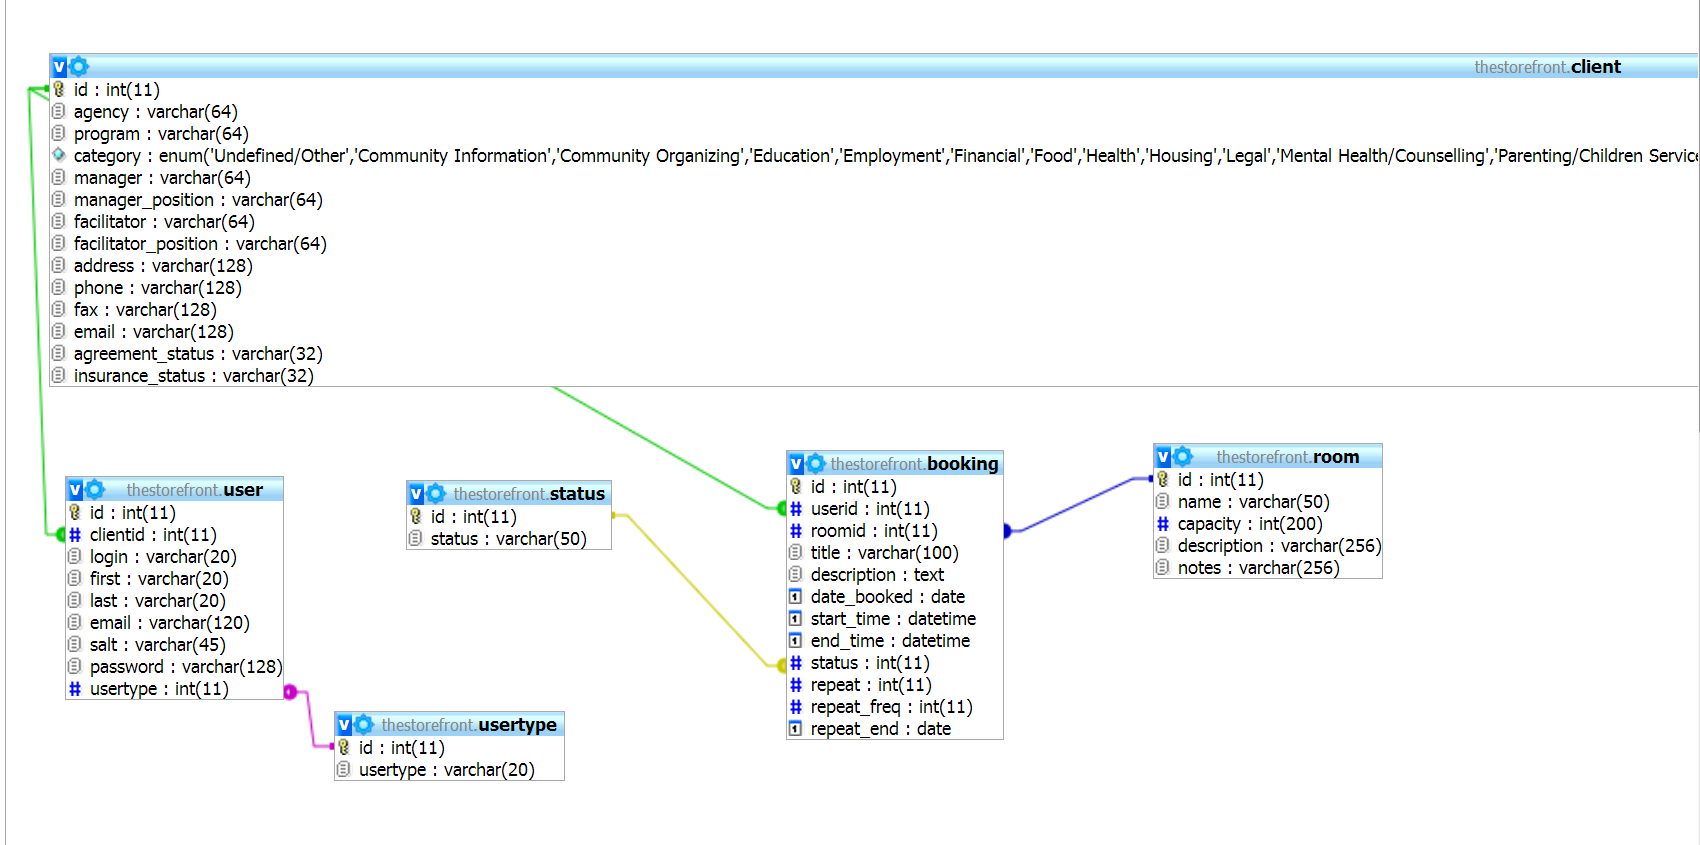
\includegraphics[width=\linewidth]{db_schema}


\subsection{Summary}

Our website uses CodeIgniter/PHP and other common web technologies with an MVC paradigm. Several internal CodeIgniter libraries were used to quickly implement functionality and reduce risk. FullCalendar and Qtip2 were also used to implement features described by our user stories. Alternatives were rejected by using user stories to determine the value of a technology. The back-end is a fully-functional MySQL server that is integrated into the application via CodeIgniter.

Our application is fully functional, has already been deployed, and is \textit{not} a mock-up.






\end{document}

